\documentclass[12pt]{article}
\linespread{1.3}
\usepackage{hyperref}
\usepackage{enumitem}
%\usepackage{enumerate}
\usepackage{changepage,lipsum,titlesec, longtable}
\usepackage{cite}
\usepackage{comment, xcolor}
\usepackage[pdftex]{graphicx}
  \graphicspath{{images/}, {images/stat/}}
  \DeclareGraphicsExtensions{.pdf,.jpeg,.png, .jpg}
\usepackage[cmex10]{amsmath}
\usepackage{tikz}
\usepackage{array} 
\usepackage{subfigure} 
\newcommand{\grey}[1]{\textcolor{black!30}{#1}}
\newcommand{\red}[1]{\textcolor{red!50}{#1}}
\newcommand{\question}[1]{\textcolor{magenta}{\textbf{Question: } {#1}}}
\newcommand{\fref}[1]{Figure~\ref{#1}}
\newcommand{\tref}[1]{Table~\ref{#1}}
\newcommand{\eref}[1]{Equation~\ref{#1}}
\newcommand{\cref}[1]{Chapter~\ref{#1}}
\newcommand{\sref}[1]{Section~\ref{#1}}
\newcommand{\aref}[1]{Appendix~\ref{#1}}
\newcommand{\note}[0]{\textbf{Note: }}

\renewcommand{\labelenumii}{\theenumii}
\renewcommand{\theenumii}{\theenumi.\\arabic{enumii}.}

\oddsidemargin0cm
\topmargin-2cm %I recommend adding these three lines to increase the
\textwidth16.5cm %amount of usable space on the page (and save trees)
\textheight23.5cm

\makeatletter
\renewcommand\paragraph{\@startsection{paragraph}{4}{\z@}%
            {-2.5ex\@plus -1ex \@minus -.25ex}%
            {1.25ex \@plus .25ex}%
            {\normalfont\normalsize\bfseries}}
\makeatother
\setcounter{secnumdepth}{4} % how many sectioning levels to assign numbers to
\setcounter{tocdepth}{4}    % how many sectioning levels to show in ToC

% draw diagram
\usetikzlibrary{shapes.geometric, arrows}
\tikzstyle{data} = [font=\scriptsize, rectangle, rounded corners, minimum width=1.5cm, minimum height=1cm,align=left, draw=black, fill=black!30]
\tikzstyle{database} = [font=\scriptsize, rectangle, rounded corners, minimum width=3cm, minimum height=1cm,align=left, draw=black, fill=green!30]
\tikzstyle{query} = [font=\scriptsize,trapezium, trapezium left angle=70, trapezium right angle=110, minimum width=0.5cm, minimum height=0.5cm, text centered, draw=black, fill=blue!30]
\tikzstyle{process} = [font=\scriptsize,rectangle, minimum width=3cm, minimum height=1cm, text centered, draw=black, fill=orange!30]
\tikzstyle{spliter} = [font=\scriptsize,diamond, minimum width=2cm, minimum height=1cm, text centered, draw=black, fill=green!30]
\tikzstyle{decision} = [font=\scriptsize,diamond, minimum width=3cm, minimum height=1cm, text centered, draw=black, fill=green!30]
\tikzstyle{arrow} = [thick,->,>=stealth]
\tikzstyle{bi-arrow} = [thick,->,>=stealth]

\begin{document}
\title{Data processing for PM data\\
       \large GSA project}
\maketitle
\tableofcontents
\newpage
\section{Introduction}\label{sec:intro}
The document records the process of calculating EUI for different
meter type for Jihyun

\section{Process}
\subsection{Convert natural gas unit to kbtu}
There are two units used in PM data:
\makeatletter
\def\verbatim@font{\linespread{1}\small\ttfamily}
\begin{verbatim}
# Gas consumption unit types
gas_unit
cf (cubic feet)    83928
therms               275

# Electric - Grid consumption unit types
elec_unit
kWh (thousand Watt-hours)    115504
\end{verbatim}
From the
\href{https://portfoliomanager.energystar.gov/pdf/reference/Thermal%20Conversions.pdf}{Energy Star PM website document}, we get the energy conversion to be:
$$1 kbtu = 1.026 cf$$
$$1 kbtu = 100 therms $$
\begin{figure}[h!]
  \centering
  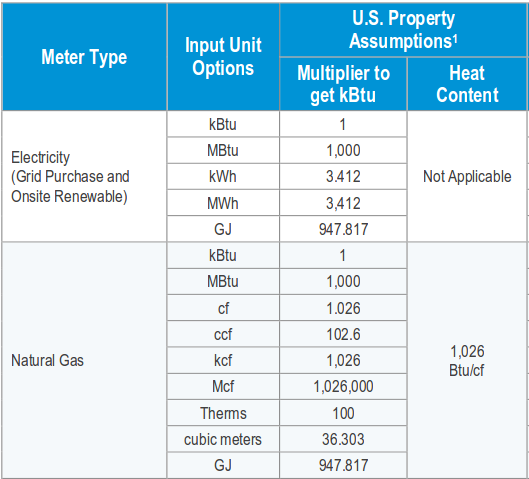
\includegraphics[width = 0.5\textwidth]{gas2kbtu.png}
  \caption{Conversion table from EnergyStar Website}
  \label{fig:gas2kbtu}
\end{figure}
The converted result is as follows
\begin{verbatim}
     gas_amt gas_unit  gas_amt_kbtu
153      NaN                    NaN
154      NaN                    NaN
155      NaN                    NaN
156      NaN                    NaN
157      NaN                    NaN
158      NaN                    NaN
159      NaN                    NaN
160      NaN                    NaN
161      NaN                    NaN
162      NaN                    NaN

[10 rows x 3 columns]
cf (cubic feet)
   gas_amt         gas_unit  gas_amt_kbtu
0  1890000  cf (cubic feet)       1939140
1  2440000  cf (cubic feet)       2503440
2  3213000  cf (cubic feet)       3296538
3  4430000  cf (cubic feet)       4545180
4  2656000  cf (cubic feet)       2725056
5  3323000  cf (cubic feet)       3409398
6  2508000  cf (cubic feet)       2573208
7  1554000  cf (cubic feet)       1594404
8  1062000  cf (cubic feet)       1089612
9   348000  cf (cubic feet)        357048

[10 rows x 3 columns]
therms
       gas_amt gas_unit  gas_amt_kbtu
24208       39   therms          3900
24209       14   therms          1400
24210       20   therms          2000
24211      209   therms         20900
24212       98   therms          9800
24213      571   therms         57100
24214      658   therms         65800
24215      113   therms         11300
24216       91   therms          9100
24217      100   therms         10000

\end{verbatim}
\subsection{Adding Gas and Electricity}
\begin{verbatim}
     elec_amt                  elec_unit  gas_amt gas_unit  gas_amt_kbtu  \
153    523200  kWh (thousand Watt-hours)      NaN                    NaN   
154     13440  kWh (thousand Watt-hours)      NaN                    NaN   
155     15880  kWh (thousand Watt-hours)      NaN                    NaN   
156     14760  kWh (thousand Watt-hours)      NaN                    NaN   
157     16800  kWh (thousand Watt-hours)      NaN                    NaN   
158     15720  kWh (thousand Watt-hours)      NaN                    NaN   
159     13600  kWh (thousand Watt-hours)      NaN                    NaN   
160     14920  kWh (thousand Watt-hours)      NaN                    NaN   
161     12080  kWh (thousand Watt-hours)      NaN                    NaN   
162     12880  kWh (thousand Watt-hours)      NaN                    NaN   

     total_amt  
153        NaN  
154        NaN  
155        NaN  
156        NaN  
157        NaN  
158        NaN  
159        NaN  
160        NaN  
161        NaN  
162        NaN  

[10 rows x 6 columns]
cf (cubic feet)
   elec_amt                  elec_unit  gas_amt         gas_unit  \
0    739200  kWh (thousand Watt-hours)  1890000  cf (cubic feet)   
1    616000  kWh (thousand Watt-hours)  2440000  cf (cubic feet)   
2    684400  kWh (thousand Watt-hours)  3213000  cf (cubic feet)   
3    714800  kWh (thousand Watt-hours)  4430000  cf (cubic feet)   
4    620400  kWh (thousand Watt-hours)  2656000  cf (cubic feet)   
5    638800  kWh (thousand Watt-hours)  3323000  cf (cubic feet)   
6    682400  kWh (thousand Watt-hours)  2508000  cf (cubic feet)   
7    719600  kWh (thousand Watt-hours)  1554000  cf (cubic feet)   
8    764800  kWh (thousand Watt-hours)  1062000  cf (cubic feet)   
9    770400  kWh (thousand Watt-hours)   348000  cf (cubic feet)   

   gas_amt_kbtu  total_amt  
0       1939140    2678340  
1       2503440    3119440  
2       3296538    3980938  
3       4545180    5259980  
4       2725056    3345456  
5       3409398    4048198  
6       2573208    3255608  
7       1594404    2314004  
8       1089612    1854412  
9        357048    1127448  

[10 rows x 6 columns]
therms
       elec_amt                  elec_unit  gas_amt gas_unit  gas_amt_kbtu  \
24208    105840  kWh (thousand Watt-hours)       39   therms          3900   
24209    107040  kWh (thousand Watt-hours)       14   therms          1400   
24210     84240  kWh (thousand Watt-hours)       20   therms          2000   
24211     60480  kWh (thousand Watt-hours)      209   therms         20900   
24212     55200  kWh (thousand Watt-hours)       98   therms          9800   
24213     58560  kWh (thousand Watt-hours)      571   therms         57100   
24214     54960  kWh (thousand Watt-hours)      658   therms         65800   
24215     64800  kWh (thousand Watt-hours)      113   therms         11300   
24216     62400  kWh (thousand Watt-hours)       91   therms          9100   
24217    121680  kWh (thousand Watt-hours)      100   therms         10000   

       total_amt  
24208     109740  
24209     108440  
24210      86240  
24211      81380  
24212      65000  
24213     115660  
24214     120760  
24215      76100  
24216      71500  
24217     131680 
\end{verbatim}
\section{Get monthly energy}
\subsection{Approach I}
The first approach is to take the month portion of the ``End Date''
field and assign the reading to that month. From this approach, the
result of some region turns out to be extremely large:
\begin{table}[h!]
\centering
\caption{Part of EUI table with Approach I in getting monthly data}
\label{my-label}
\begin{tabular}{llll}
Building ID & EUI              & Region & Year \\
  \hline
DC0001ZZ    & 12480.6184600518 & 11     & 2005 \\
DC0001ZZ    & 12038.598586171  & 11     & 2010 \\
DC0001ZZ    & 12037.9492157888 & 11     & 2003 \\
DC0001ZZ    & 11914.3922932142 & 11     & 2007 \\
DC0001ZZ    & 11889.482612042  & 11     & 2004 \\
DC0001ZZ    & 11490.2126073281 & 11     & 2009 \\
DC0001ZZ    & 11361.4174523634 & 11     & 2008 \\
DC0001ZZ    & 11306.0507623555 & 11     & 2006 \\
DC0001ZZ    & 10102.4922489585 & 11     & 2012 \\
DC0001ZZ    & 10029.6403215708 & 11     & 2013 \\
DC0001ZZ    & 9725.82060821062 & 11     & 2011 \\
DC0001ZZ    & 9224.79333462762 & 11     & 2014 \\
DC0001ZZ    & 9013.01753152796 & 11     & 2015 \\
DC0001ZZ    & 3764.92990668652 & 11     & 2002 \\
NY0234ZZ    & 1457.3329074403  & 2      & 2009 \\
NY0234ZZ    & 1451.37965153371 & 2      & 2008
\end{tabular}
\end{table}

The box plot is as follows, we can see a lot of outliers with very large EUI
\begin{figure}[h!]
  \centering
  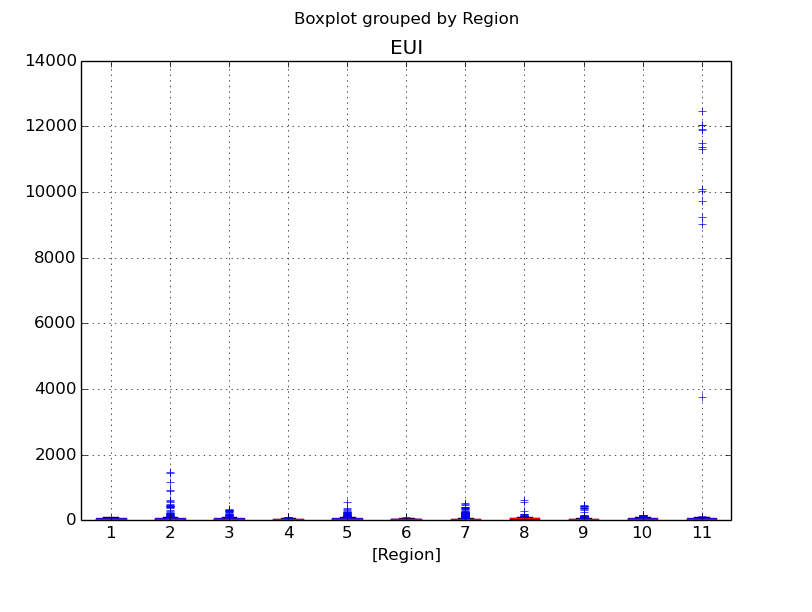
\includegraphics[width = 0.5\textwidth]{eui_1.png}
  \caption{EUI by region, using Approach I in getting month data}
  \label{fig:eui_1}
\end{figure}

The problem is there are multiple records for a month. For example,
for building 20600, there are two records for Aug-2012 (Aug-02-2012 and Aug-. The way the
table with the desired form that there are individual columns for
different meter type is generated as follows: the data of is grouped
according to the value of the field ``Meter Type'', then the groups of
energy consumption type is ``joined'' on ``Portfolio Manager ID'', ``Year'', and ``Month''. Thus if there are two Aug-2012 records 
 \begin{table}[h!]
\centering
\caption{Example of two records for one month}
\label{my-label}
\begin{tabular}{p{2cm}p{3cm}lll}
Portfolio Manager ID & Portfolio Manager Meter ID & Meter Type  &  End Date            & Usage/Quantity  \\
  \hline
20600                & 4717275                    & Natural Gas &  2012-Aug-02 0:00:00 & 13752           \\
20600                & 4717275                    & Natural Gas &  2012-Aug-30 0:00:00 & 80123          
\end{tabular}
\end{table}

\subsection{Approach II}
I have considered another approach: for a date mm-dd-yyyy, if dd < 15,
month = mm, else month = mm + 1 This doesn't work, because there are
also cases like building 20597 which has the following pattern of
record time: 2010-Jul-31, 2010-Aug-31, 2010-Sep-06 In this case, there
will still be two records of Aug.  The next thought could be to
calculate the time difference between adjacent rows and creating
symbolic months. This will not give the right answer either
considering the above example.

\subsection{Approach III}
If there are two or more records in a month, sum up the value of the records. In Pandas, it is achieved by ``resample'' to the month interval and aggregate the results with ``sum'' method.

\section{EUI graphs}
\subsection{By region alone}
\begin{figure}[h!]
  \centering
  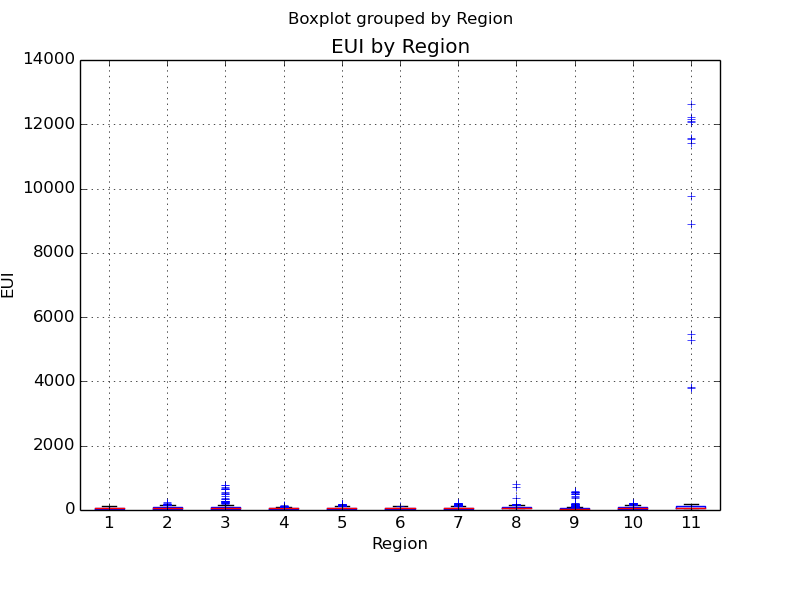
\includegraphics[width = 0.8\textwidth]{EUIbyRegion.png}
  \caption{EUI by region}
  \label{fig:EuibyRegion}
\end{figure}

\begin{figure}[h!]
  \centering
  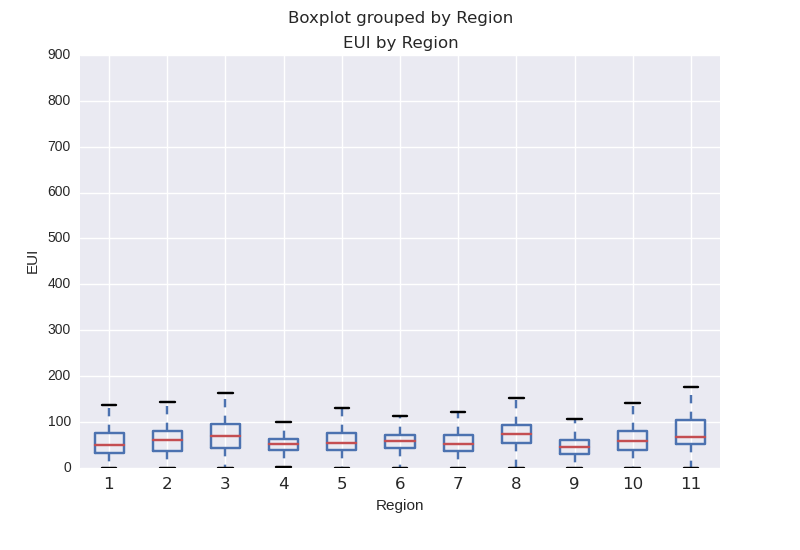
\includegraphics[width = 0.8\textwidth]{EUIbyRegion-noDC0001ZZ.png}
  \caption{EUI by region, excluding a building with extremely high energy consumption, DC0001ZZ}
  \label{fig:EuibyRegion-noDC0001ZZ}
\end{figure}

\begin{figure}[h!]
  \centering
  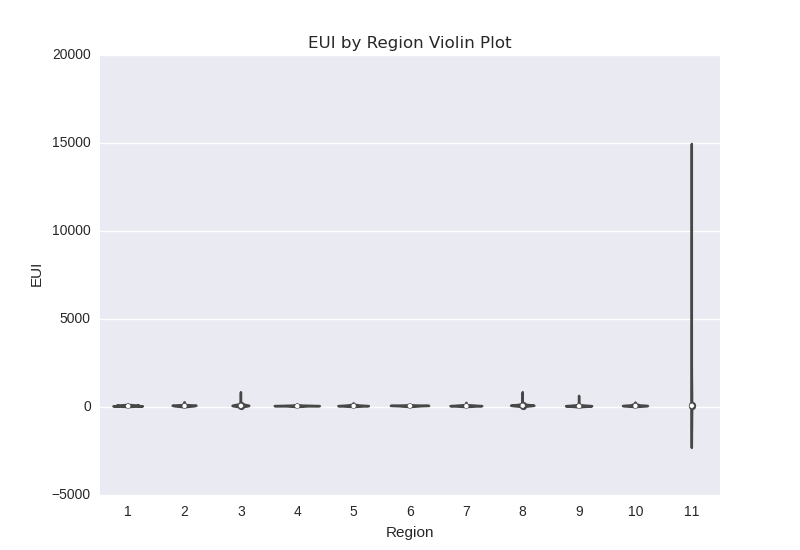
\includegraphics[width = 0.8\textwidth]{EUIbyRegionViolin.png}
  \caption{EUI by region violin plot}
  \label{fig:EuibyRegionViolin}
\end{figure}

\begin{figure}[h!]
  \centering
  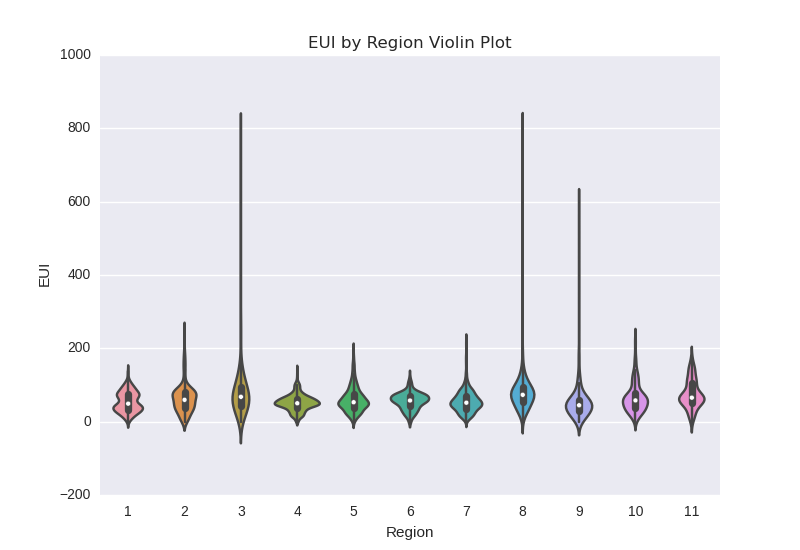
\includegraphics[width = 0.8\textwidth]{EUIbyRegionViolin-noDC0001ZZ.png}
  \caption{EUI by region violin plot, excluding a building with extremely high energy consumption, DC0001ZZ}
  \label{fig:EuibyRegionViolin-noDC0001ZZ}
\end{figure}

\newpage
\bibliographystyle{plain} \bibliography{myCitation}
\end{document}
